\documentclass[paper=a4, fontsize=11pt]{scrartcl} % A4 paper and 11pt font size
\usepackage[T1]{fontenc} % Use 8-bit encoding that has 256 glyphs
\usepackage[english]{babel} 
\usepackage{amsmath,amsfonts,amsthm} 
\usepackage{graphicx}
\usepackage{caption}
\usepackage{subcaption}
\usepackage{float}
\numberwithin{figure}{section} 
\setlength\parindent{0pt} % Removes all indentation from paragraphs - comment this line for an assignment with lots of text


\title{	
\normalfont \normalsize 
\textsc{Practical exercise with ARTS, OSF SoSe16} \\ [25pt] % Your university, school and/or department name(s)
%\horrule{0.5pt} \\[0.4cm] % Thin top horizontal rule
\huge Exercise 4: Outgoing Longwave Radiation \\ % The assignment title
}

\author{sample solution}
\date{\normalsize\today} 

\begin{document}

\maketitle

1. Run arts on the controlfile $“olr.arts”$. This will calculate the spectrum of outgoing 
longwave radiation (OLR) for a midlatitude-summer atmosphere. The calculation has been simplified, 
so that you do not have to wait so long for the results. For example, we use only water vapor and 
carbon dioxide as absorbers. We use only 1000 frequency grid points and approximately 54,000 spectral 
lines, whereas for accurate calculations one needs at least 10,000 frequency grid points and 500,000 
spectral lines, taking into account absorbing species like ozone and methane.\ \\

2. Use the Matlab program $plot\_olr$ to display the results. This time the radiances 
are shown in SI units, not in brightness temperature.  Planck curves for different temperatures are 
shown for comparison. The number shown is the area under the curve. If this is integrated over 
direction (one hemisphere) it is the power that the atmosphere looses to space per square meter. \ \\

\begin{itemize}
	\item How would the OLR spectrum look in units of brightness temperature?
	\item How would the Planck curves look in units of brightness temperature?
	\item Find the CO2 absorption band and the regions of H2O absorption (ask the teacher 
	    to point them out to you). Where in the atmosphere does the radiation in the CO2 band originate? 
	\item Are there window regions? What will determine the OLR in the window regions?
	\item Use the plot to explain the atmospheric greenhouse effect to your neighbor. \ \\
\end{itemize}

\begin{figure}[H]
\centering
	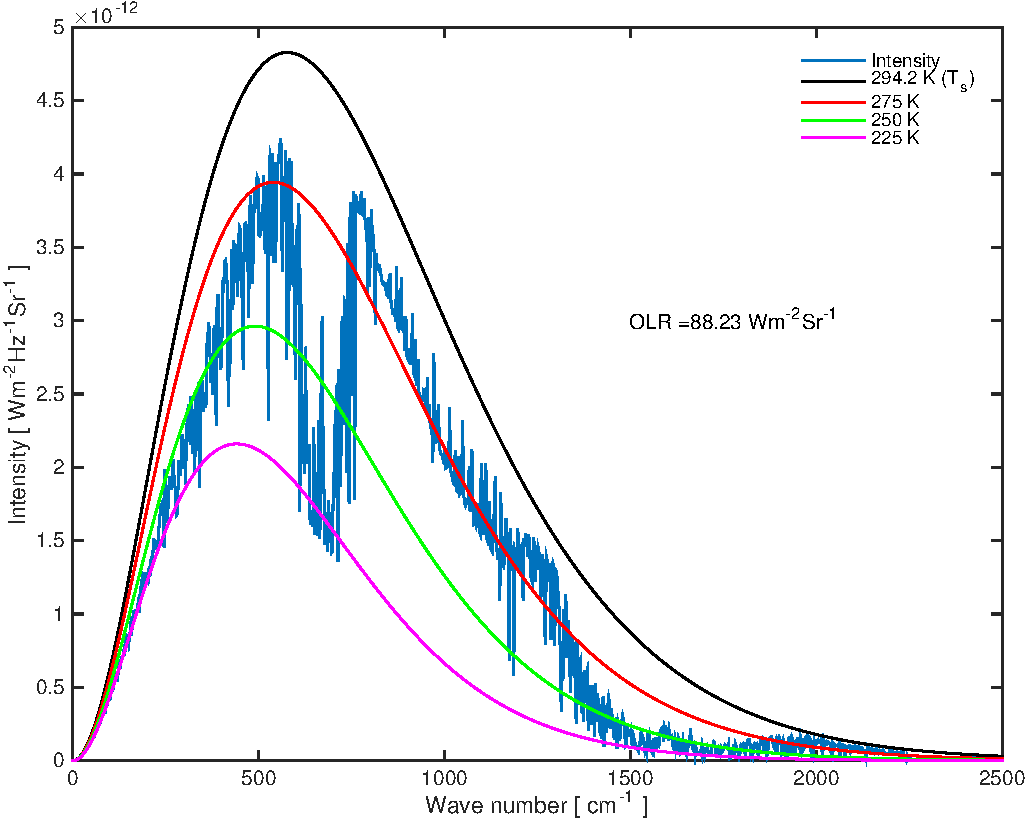
\includegraphics[width=0.9\textwidth]{plots/olr.pdf}
	\caption{spectrum of outgoing longwave radiation and Planck curves for different temperatures}
\end{figure}

3. An interesting question is how the OLR changes if the atmospheric composition changes. 
You can investigate this by modifying the ARTS controlfile. The place to do this 
is below line 76, where it says “Atmospheric scenario for midlatitude summer”. 
By adjusting the path ``./midlatitude-summer/midlatitude-summer'' 
you can make changes to the atmospheric composition. There are three possibilities:
%\begin{addmargin}[2]
\begin{itemize}
	\item Add 1 K to the temperature: \\ ``./midlatitude-summer\_+T/midlatitude-summer''
	\item Multiply the $CO_{2}$ concentration by 2: \\ ``./midlatitude-summer\_+CO2/midlatitude-summer''
	\item Multiply the $H_{2}O$ concentration by 1.2: \\ ``./midlatitude-summer\_+H2O/midlatitude-summer'' \ \\
\end{itemize}
%\end{addmargin}

Each group should investigate one parameter. Change it, and calculate the spectrum, then make a plot. 

\begin{figure}[H]
\centering
	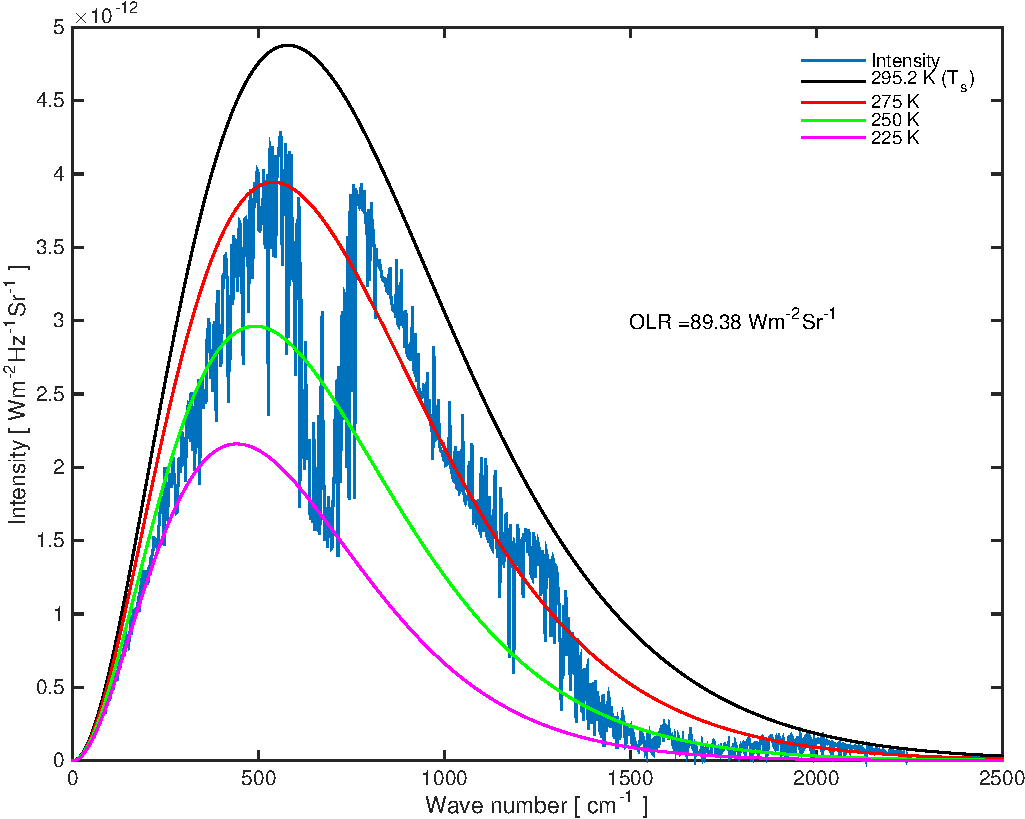
\includegraphics[width=0.7\textwidth]{plots/olr_+T.pdf}
	\caption{spectrum of outgoing longwave radiation for higher Temperature (+1K)}
\end{figure}

\begin{figure}[H]
\centering
	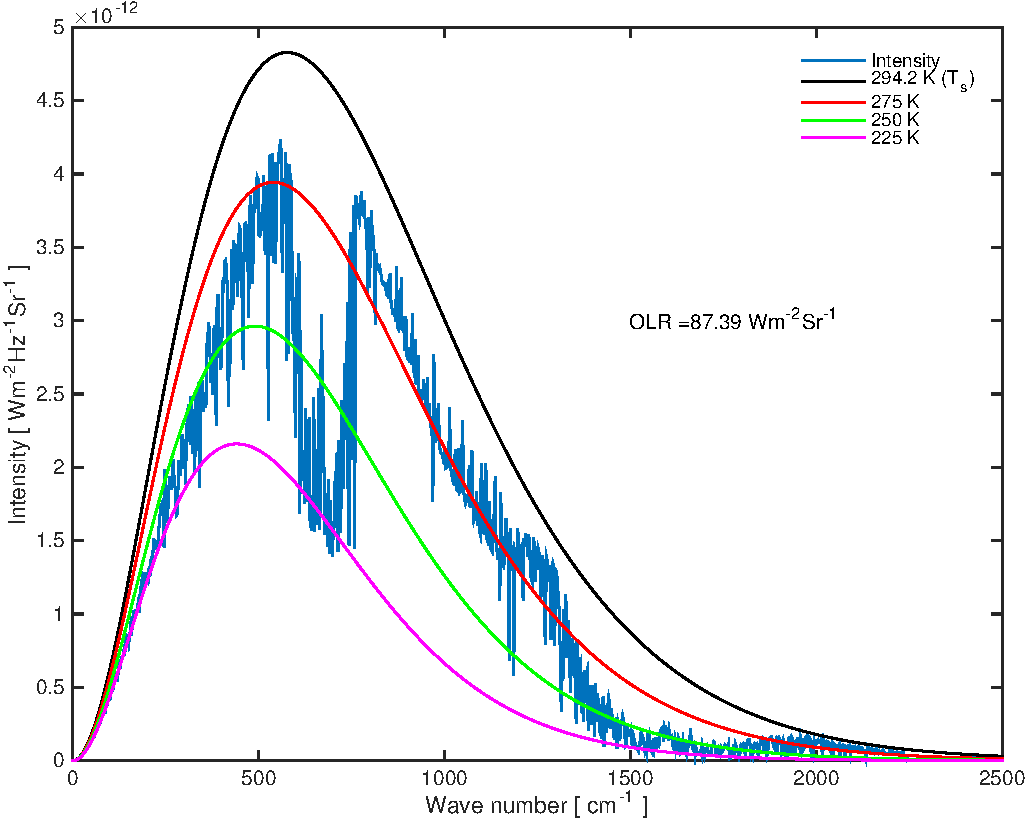
\includegraphics[width=0.7\textwidth]{plots/olr_+CO2.pdf}
	\caption{spectrum of outgoing longwave radiation for higher $CO_{2}$ concentration}
\end{figure}

\begin{figure}[H]
\centering
	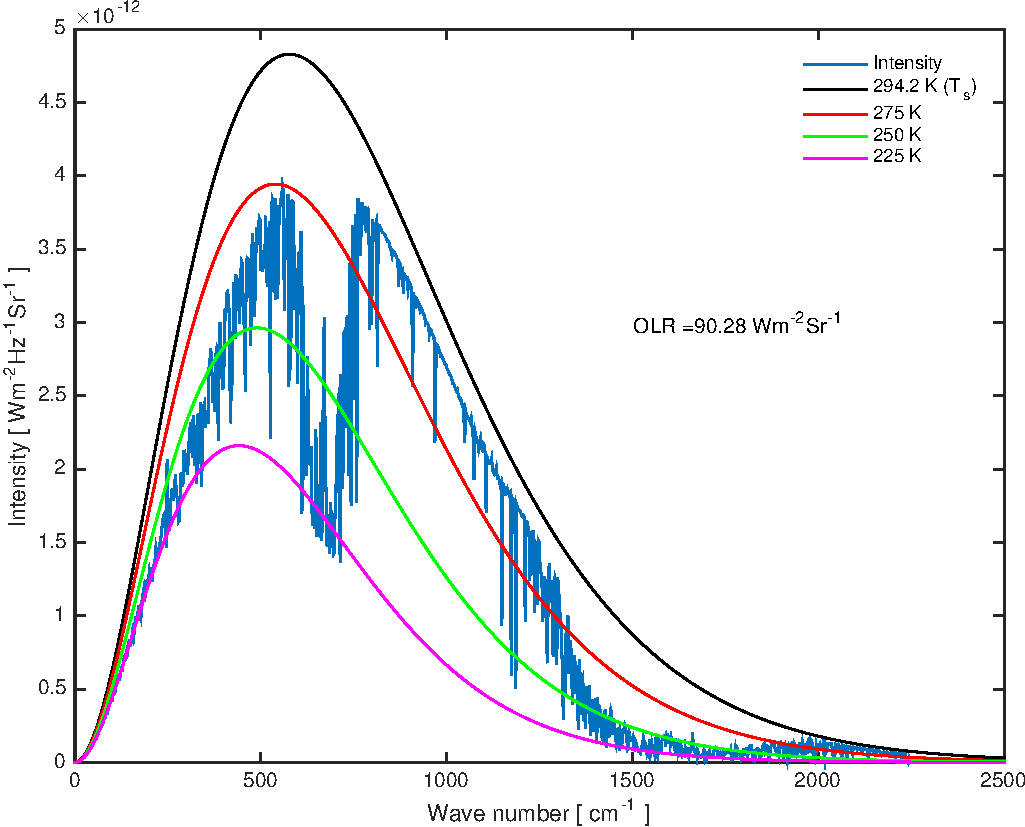
\includegraphics[width=0.7\textwidth]{plots/olr_+H2O.pdf}
	\caption{spectrum of outgoing longwave radiation for higher $H_{2}O$ concentration}
\end{figure}

\begin{itemize}
	\item Compare the spectra for humidity and carbon dioxide changes. Where do the changes occur?
	\item Compare the OLR numbers, which is the more potent greenhouse gas, $CO_{2}$ or $H_{2}O$?
	\item What is the effect of the temperature change? Explain.
\end{itemize}

\end{document}
